% !TEX TS-program = xelatex
% Command for running this example (needs latexmkrc file):
%    latexmk -bibtex -pdf main.tex

%	نمونه پایان‌نامه آماده شده با استفاده از کلاس tehran-thesis، نگارش 1
%	سینا ممکن، دانشگاه تهران 
%	https://github.com/sinamomken/tehran-thesis
%	گروه پارسی‌لاتک
%	http://www.parsilatex.com
%	این نسخه، بر اساس نسخه‌ 0.1 از کلاس IUST-Thesis آقای محمود امین‌طوسی آماده شده است.
%        http://profsite.sttu.ac.ir/mamintoosi

%----------------------------------------------------------------------------------------------
% اگر قصد نوشتن پروژه کارشناسی را دارید، در خط زیر به جای msc، کلمه bsc و اگر قصد نوشتن رساله دکترا را دارید، کلمه phd را قرار دهید. کلیه تنظیمات لازم، به طور خودکار، اعمال می‌شود.

% اگر مایلید پایان‌نامه شما دورو باشد به جای oneside در خط زیر از twoside استفاده کنید.

% برای حاشیه‌نویسی و کم کردن صفحات ابتدایی، گزینه draft را وارد و برای نسخه نهایی آن را حذف کنید.

% برای استفاده از قلم‌های سری IR Series گزینه irfonts را وارد و برای استفاده از قلم‌های X Series 2 آن را حذف کنید.

\documentclass[
oneside
% ,openany
,bsc
,irfonts
% ,draft
]{./tex/tehran-thesis}

% فایل commands.tex را مطالعه کنید؛ چون دستورات مربوط به فراخوانی بسته‌ها، فونت و دستورات خاص در این فایل قرار دارد.
% در این فایل، دستورها و تنظیمات مورد نیاز، آورده شده است.
%-------------------------------------------------------------------------------------------------------------------
% دستوراتی که پوشه پیش‌فرض زیرفایل‌های tex را مشخص می‌کند.
%\makeatletter
%\def\input@path{{./tex/}}
%\makeatother
% در ورژن جدید زی‌پرشین برای تایپ متن‌های ریاضی، این سه بسته، حتماً باید فراخوانی شود
\usepackage{amsthm,amssymb,amsmath}
% بسته‌ای برای تنطیم حاشیه‌های بالا، پایین، چپ و راست صفحه
\usepackage[a4paper, top=40mm, bottom=40mm, outer=25mm, inner=35mm]{geometry}
% بسته‌‌ای برای ظاهر شدن شکل‌ها و تعیین آدرس تصاویر
\usepackage[final]{graphicx}
\graphicspath{{./img/}}
% بسته‌های مورد نیاز برای نوشتن کدها، رنگ‌آمیزی آنها و تعیین پوشهٔ کدها
\usepackage[final]{listings}
\usepackage[usenames,dvipsnames,svgnames,table]{xcolor}
\lstset{inputpath=./code/}
% بسته‌ای برای رسم کادر
\usepackage{framed} 
% بسته‌‌ای برای چاپ شدن خودکار تعداد صفحات در صفحه «معرفی پایان‌نامه»
\usepackage{lastpage}
% بسته‌ٔ لازم برای: ۱. تغییر شماره‌گذاری صفحات پیوست. ۲. تصحیح باگ آدرس وب حاوی '%' در مراجع
\usepackage{etoolbox}

%%%%%%%%%%%%%%%%%%%%%%%%%%%%%%%%%%%%
%%% دستورات وابسته به استیل مراجع:
%% اگر از استیل‌های natbib (plainnat-fa، asa-fa، chicago-fa) استفاده می‌کنید، خط زیر را فعال و بعدی‌اش را غیرفعال کنید.
%\usepackage{natbib}
%\newcommand{\citelatin}[1]{\cite{#1}\LTRfootnote{\citeauthor*{#1}}}
%\newcommand{\citeplatin}[1]{\citep{#1}\LTRfootnote{\citeauthor*{#1}}}
%% اگر از سایر استیل‌ها استفاده می‌کنید، خط بالا را غیرفعال و خط‌های زیر را فعال کنید.
\let\citep\cite
\let\citelatin\cite
\let\citeplatin\cite
%%%%%%%%%%%%
% بررسی حالت پیش نویس
\usepackage{ifdraft}
\ifdraft
{%
	% بسته‌ٔ ایجاد لینک‌های رنگی با امکان جهش
	\usepackage[unicode=true,pagebackref=true,
colorlinks,linkcolor=blue,citecolor=blue,final]{hyperref}
	%\usepackage{todonotes}
	\usepackage[firstpage]{draftwatermark}
	\SetWatermarkText{\ \ \ \rl{پیش‌نویس}}
	\SetWatermarkScale{1.2}
}
{ 
	\usepackage[pagebackref=false]{hyperref}
	%\usepackage[disable]{todonotes} % final without TODOs
}

\usepackage[obeyDraft]{todonotes}
\setlength{\marginparwidth}{2cm}

%%%%%%%%%%%%
%%% تصحیح باگ: اگر در مراجع، آدرس وب حاوی '%' بوده و pagebackref فعال باشد، دستورات زیر باید بیایند:
%% برای استیل‌های natbib مثل plainnat-fa، asa-fa، chicago-fa
\makeatletter
\let\ORIG@BR@@lbibitem\BR@@lbibitem
\apptocmd\ORIG@BR@@lbibitem{\endgroup}{}{}
\def\BR@@lbibitem{\begingroup\catcode`\%=12 \ORIG@BR@@lbibitem}
\makeatother
%% برای سایر استیل‌ها
\makeatletter
\let\ORIG@BR@@bibitem\BR@@bibitem
\apptocmd\ORIG@BR@@bibitem{\endgroup}{}{}
\def\BR@@bibitem{\begingroup\catcode`\%=12 \ORIG@BR@@bibitem}
\makeatother
%%%%%%%%%%%%%%%%%%%%%%%%%%%%%%%%%%%%

% بسته‌ لازم برای تنظیم سربرگ‌ها
\usepackage{fancyhdr}
%\usepackage{enumitem}
\usepackage{setspace}
% بسته‌های لازم برای نوشتن الگوریتم
\usepackage{algorithm}
\usepackage{algorithmic}
% بسته‌های لازم برای رسم بهتر جداول
\usepackage{tabulary}
\usepackage{tabularx}
\usepackage{rotating}
% بسته‌های لازم برای رسم تنظیم بهتر شکل‌ها و زیرشکل‌ها
\usepackage[export]{adjustbox}
\usepackage{subfig}
\usepackage[subfigure]{tocloft}
% بسته‌ای برای رسم نمودارها و نیز صفحه مالکیت اثر
\usepackage{tikz}
% بسته‌ای برای ظاهر شدن «مراجع» و «نمایه» در فهرست مطالب
\usepackage[nottoc]{tocbibind}
% دستورات مربوط به ایجاد نمایه
\usepackage{makeidx}
\makeindex
%%% بسته ایجاد واژه‌نامه با xindy
\usepackage[xindy,toc,acronym,nonumberlist=true]{glossaries}

% بسته‌ای برای افزودن تورفتگی به ابتدای اولین پاراگراف هر بخش
\usepackage{indentfirst}

% بسته زیر باگ ناشی از فراخوانی بسته‌های زیاد را برطرف می‌کند.
\usepackage{morewrites}
%%%%%%%%%%%%%%%%%%%%%%%%%%
% فراخوانی بسته زی‌پرشین (باید آخرین بسته باشد)
\usepackage[extrafootnotefeatures, localise=on, displaymathdigits=persian]{xepersian}




\makeatletter
% تعریف قلم فارسی و انگلیسی و مکان قلم‌ها
\if@irfonts
\settextfont[Path={./font/}, BoldFont={IRLotusICEE_Bold.ttf}, BoldItalicFont={IRLotusICEE_BoldIranic.ttf}, ItalicFont={IRLotusICEE_Iranic.ttf},Scale=1.2]{IRLotusICEE.ttf}
% LiberationSerif or FreeSerif as free equivalents of Times New Roman
\setlatintextfont[Path={./font/}, BoldFont={LiberationSerif-Bold.ttf}, BoldItalicFont={LiberationSerif-BoldItalic.ttf}, ItalicFont={LiberationSerif-Italic.ttf},Scale=1]{LiberationSerif-Regular.ttf}
% چنانچه می‌خواهید اعداد در فرمول‌ها، انگلیسی باشد، خط زیر را غیرفعال کنید
% و گزینهٔ displaymathdigits=persian را از خط ۱۰۹ حذف کنید.
\setdigitfont[Path={./font/}, Scale=1.2]{IRLotusICEE.ttf}
% تعریف قلم‌های فارسی و انگلیسی اضافی برای استفاده در بعضی از قسمت‌های متن
\setiranicfont[Path={./font/}, Scale=1.3]{IRLotusICEE_Iranic.ttf}				% ایرانیک، خوابیده به چپ
\setmathsfdigitfont[Path={./font/}]{IRTitr.ttf}
\defpersianfont\titlefont[Path={./font/}, Scale=1]{IRTitr.ttf}
% برای تعریف یک قلم خاص عنوان لاتین، خط بعد را فعال و ویرایش کنید و خط بعد از آن را غیرفعال کنید.
% \deflatinfont\latintitlefont[Scale=1]{LiberationSerif}
\font\latintitlefont=cmssbx10 scaled 2300 %cmssbx10 scaled 2300
\else
\settextfont{XB Niloofar}
\setlatintextfont{Junicode}
% چنانچه می‌خواهید اعداد در فرمول‌ها، انگلیسی باشد، خط زیر را غیرفعال کنید
% و گزینهٔ displaymathdigits=persian را از خط ۱۰۹ حذف کنید.
\setdigitfont{XB Niloofar}
% تعریف قلم‌های فارسی و انگلیسی اضافی برای استفاده در بعضی از قسمت‌های متن
% \setmathsfdigitfont{XB Titre}
\defpersianfont\titlefont{XB Titre}
\deflatinfont\latintitlefont[Scale=1.1]{Junicode}
\fi
\makeatother

% برای استفاده از قلم نستعلیق خط بعد را فعال کنید.
% \defpersianfont\nastaliq[Scale=1.2]{IranNastaliq}


%%%%%%%%%%%%%%%%%%%%%%%%%%
% راستچین شدن todonotes
\presetkeys{todonotes}{align=right,textdirection=righttoleft}{}
\makeatletter
\providecommand\@dotsep{5}
\def\listtodoname{فهرست کارهای باقیمانده}
\def\listoftodos{\noindent{\Large\vspace{10mm}\textbf{\listtodoname}}\@starttoc{tdo}}
\renewcommand{\@todonotes@MissingFigureText}{شکل}
\renewcommand{\@todonotes@MissingFigureUp}{شکل}
\renewcommand{\@todonotes@MissingFigureDown}{جاافتاده}
\makeatother
% دستوری برای حذف کلمه «چکیده»
% \renewcommand{\abstractname}{}
% دستوری برای حذف کلمه «abstract»
%\renewcommand{\latinabstract}{}
% دستوری برای تغییر نام کلمه «اثبات» به «برهان»
\renewcommand\proofname{\textbf{برهان}}
% دستوری برای تغییر نام کلمه «کتاب‌نامه» به «مراجع»
\renewcommand{\bibname}{مراجع}
% دستوری برای تعریف واژه‌نامه انگلیسی به فارسی
\newcommand\persiangloss[2]{#1\dotfill\lr{#2}\\}
% دستوری برای تعریف واژه‌نامه فارسی به انگلیسی 
\newcommand\englishgloss[2]{#2\dotfill\lr{#1}\\}
% تعریف دستور جدید «\پ» برای خلاصه‌نویسی جهت نوشتن عبارت «پروژه/پایان‌نامه/رساله»
\newcommand{\پ}{پروژه/پایان‌نامه/رساله }

%\newcommand\BackSlash{\char`\\}

%%%%%%%%%%%%%%%%%%%%%%%%%%
% \SepMark{-}

% تعریف و نحوه ظاهر شدن عنوان قضیه‌ها، تعریف‌ها، مثال‌ها و ...
\theoremstyle{definition}
\newtheorem{definition}{تعریف}[section]
\theoremstyle{theorem}
\newtheorem{theorem}[definition]{قضیه}
\newtheorem{lemma}[definition]{لم}
\newtheorem{proposition}[definition]{گزاره}
\newtheorem{corollary}[definition]{نتیجه}
\newtheorem{remark}[definition]{ملاحظه}
\theoremstyle{definition}
\newtheorem{example}[definition]{مثال}

%\renewcommand{\theequation}{\thechapter-\arabic{equation}}
%\def\bibname{مراجع}
\numberwithin{algorithm}{chapter}
\def\listalgorithmname{فهرست الگوریتم‌ها}
\def\listfigurename{فهرست تصاویر}
\def\listtablename{فهرست جداول}

% دستور های لازم برای تعریف ترجمهٔ دستورات الگوریتم
\makeatletter
\renewcommand{\algorithmicrequire}{\if@RTL\textbf{ورودی:}\else\textbf{Require:}\fi}
\renewcommand{\algorithmicensure}{\if@RTL\textbf{خروجی:}\else\textbf{Ensure:}\fi}
\renewcommand{\algorithmicend}{\if@RTL\textbf{پایان}\else\textbf{end}\fi}
\renewcommand{\algorithmicif}{\if@RTL\textbf{اگر}\else\textbf{if}\fi}
\renewcommand{\algorithmicthen}{\if@RTL\textbf{آنگاه}\else\textbf{then}\fi}
\renewcommand{\algorithmicelse}{\if@RTL\textbf{وگرنه}\else\textbf{else}\fi}
\renewcommand{\algorithmicfor}{\if@RTL\textbf{برای}\else\textbf{for}\fi}
\renewcommand{\algorithmicforall}{\if@RTL\textbf{برای هر}\else\textbf{for all}\fi}
\renewcommand{\algorithmicdo}{\if@RTL\textbf{انجام بده}\else\textbf{do}\fi}
\renewcommand{\algorithmicwhile}{\if@RTL\textbf{تا زمانی که}\else\textbf{while}\fi}
\renewcommand{\algorithmicloop}{\if@RTL\textbf{تکرار کن}\else\textbf{loop}\fi}
\renewcommand{\algorithmicrepeat}{\if@RTL\textbf{تکرار کن}\else\textbf{repeat}\fi}
\renewcommand{\algorithmicuntil}{\if@RTL\textbf{تا زمانی که}\else\textbf{until}\fi}
\renewcommand{\algorithmicprint}{\if@RTL\textbf{چاپ کن}\else\textbf{print}\fi}
\renewcommand{\algorithmicreturn}{\if@RTL\textbf{بازگردان}\else\textbf{return}\fi}
\renewcommand{\algorithmicand}{\if@RTL\textbf{و}\else\textbf{and}\fi}
\renewcommand{\algorithmicor}{\if@RTL\textbf{و یا}\else\textbf{or}\fi} % TODO add better translate
\renewcommand{\algorithmicxor}{\if@RTL\textbf{یا}\else\textbf{xor}\fi} % TODO add better translate
\renewcommand{\algorithmicnot}{\if@RTL\textbf{نقیض}\else\textbf{not}\fi}
\renewcommand{\algorithmicto}{\if@RTL\textbf{تا}\else\textbf{to}\fi}
\renewcommand{\algorithmicinputs}{\if@RTL\textbf{ورودی‌ها}\else\textbf{inputs}\fi}
\renewcommand{\algorithmicoutputs}{\if@RTL\textbf{خروجی‌ها}\else\textbf{outputs}\fi}
\renewcommand{\algorithmicglobals}{\if@RTL\textbf{متغیرهای عمومی}\else\textbf{globals}\fi}
\renewcommand{\algorithmicbody}{\if@RTL\textbf{انجام بده}\else\textbf{do}\fi}
\renewcommand{\algorithmictrue}{\if@RTL\textbf{درست}\else\textbf{true}\fi}
\renewcommand{\algorithmicfalse}{\if@RTL\textbf{نادرست}\else\textbf{false}\fi}
\renewcommand{\algorithmicendif}{\algorithmicend\textbf{ شرط }\algorithmicif}
\renewcommand{\algorithmicendfor}{\algorithmicend\textbf{ حلقهٔ }\algorithmicfor}
\renewcommand{\algorithmicendwhile}{\algorithmicend\textbf{ حلقهٔ }\algorithmicwhile}
\renewcommand{\algorithmicendloop}{\algorithmicend\textbf{ حلقهٔ }\algorithmicloop}
\renewcommand{\algorithmiccomment}[1]{\{{\itshape #1}\}}
\makeatletter

%%%%%%%%%%%%%%%%%%%%%%%%%%%%
%%% دستورهایی برای سفارشی کردن سربرگ صفحات:
%\newcommand{\SetHeader}[1]{
% دستور زیر معادل با گزینه twoside است.
%\csname@twosidetrue\endcsname
\pagestyle{fancy}
%% دستورات زیر سبک صفحات fancy را تغییر می‌دهد:
% O=Odd, E=Even, L=Left, R=Right
% در صورت oneside بودن، عنوان فصل، سمت چپ ظاهر می‌شود.
\fancyhead{}
\fancyhead[OL]{\small\leftmark}
\fancyhead[ER]{\small\leftmark}
\fancyhead[OR]{\footnotesize\rightmark}
\fancyhead[EL]{\footnotesize\rightmark}
\renewcommand{\headrulewidth}{0.75pt}
% شکل‌دهی شماره و عنوان فصل در سربرگ
\renewcommand{\chaptermark}[1]{\markboth{فصل~\thechapter:\ #1}{}}
\makeatletter
\renewcommand{\rightmark}[1]{\@title}
\makeatother
%}
%%%%%%%%%%%%%%%%%%%%%%%%%%%%
%\def\MATtextbaseline{1.5}
%\renewcommand{\baselinestretch}{\MATtextbaseline}
\doublespacing
%%%%%%%%%%%%%%%%%%%%%%%%%%%%%
% دستوراتی برای اضافه کردن کلمه «فصل» در فهرست مطالب

\newlength\mylenprt
\newlength\mylenchp
\newlength\mylenapp

\renewcommand\cftpartpresnum{\partname~}
\renewcommand\cftchappresnum{\chaptername~}
\renewcommand\cftchapaftersnum{:}

\settowidth\mylenprt{\cftpartfont\cftpartpresnum\cftpartaftersnum}
\settowidth\mylenchp{\cftchapfont\cftchappresnum\cftchapaftersnum}
\settowidth\mylenapp{\cftchapfont\appendixname~\cftchapaftersnum}
\addtolength\mylenprt{\cftpartnumwidth}
\addtolength\mylenchp{\cftchapnumwidth}
\addtolength\mylenapp{\cftchapnumwidth}

\setlength\cftpartnumwidth{\mylenprt}
\setlength\cftchapnumwidth{\mylenchp}	

\makeatletter
{\def\thebibliography#1{\chapter*{\refname\@mkboth
   {\uppercase{\refname}}{\uppercase{\refname}}}\list
   {[\arabic{enumi}]}{\settowidth\labelwidth{[#1]}
   \rightmargin\labelwidth
   \advance\rightmargin\labelsep
   \advance\rightmargin\bibindent
   \itemindent -\bibindent

   \listparindent \itemindent
   \parsep \z@
   \usecounter{enumi}}
   \def\newblock{}
   \sloppy
   \sfcode`\.=1000\relax}}
   
%اگر مایلید در شماره گذاری حرفی و ابجد به جای آ از الف استفاده شود دستورات زیر را فعال کنید.   
%\def\@Abjad#1{%
%  \ifcase#1\or الف\or ب\or ج\or د%
%           \or هـ\or و\or ز\or ح\or ط%
%           \or ی\or ک\or ل\or م\or ن%
%           \or س\or ع\or ف\or ص%
%           \or ق\or ر\or ش\or ت\or ث%
%            \or خ\or ذ\or ض\or ظ\or غ%
%            \else\@ctrerr\fi}
%
% \def\abj@num@i#1{%
%   \ifcase#1\or الف\or ب\or ج\or د%
%            \or هـ‍\or و\or ز\or ح\or ط\fi

%   \ifnum#1=\z@\abjad@zero\fi}   
%  
%   \def\@harfi#1{\ifcase#1\or الف\or ب\or پ\or ت\or ث\or

% ج\or چ\or ح\or خ\or د\or ذ\or ر\or ز\or ژ\or س\or ش\or ص\or ض\or ط\or ظ\or ع\or غ\or

% ف\or ق\or ک\or گ\or ل\or م\or ن\or و\or ه\or ی\else\@ctrerr\fi}

%
\makeatother

%%% امکان درج کد در سند
% در این قسمت رنگ، قلم و قالب‌بندی قسمت‌های مختلف یک کد تعیین می‌شود. 
\lstdefinestyle{myStyle}{
	basicstyle=\ttfamily, % whole listing /w verbatim font
	keywordstyle=\color{blue}\bfseries, % bold black keywords
	identifierstyle=, % nothing happens
	commentstyle=\color{LimeGreen}, % green comments
	stringstyle=\ttfamily\color{red}, % red typewriter font for strings
	showstringspaces=false % no special string spaces
	breaklines=true,
	breakatwhitespace=false,
	numbers=right, % line number formats
	numberstyle=\footnotesize\lr,
	numbersep=-10pt,
	frame=single,
	captionpos=b,
	captiondirection=RTL
}
\lstset{style=myStyle} % command to set default style
\def\lstlistingname{\rl{برنامهٔ}}
\def\lstlistlistingname{\rl{فهرست برنامه‌ها}}


% for numbering subsubsections
\setcounter{secnumdepth}{3}
%to include subsubsections in the table of contents
\setcounter{tocdepth}{3}

\makeatletter
\renewcommand{\p@subfigure}{\thefigure.}
\makeatother


% مشخصات پایان‌نامه را در فایلهای faTitle و enTitle وارد نمایید.
% !TeX root=../main.tex
% در این فایل، عنوان پایان‌نامه، مشخصات خود، متن تقدیمی‌، ستایش، سپاس‌گزاری و چکیده پایان‌نامه را به فارسی، وارد کنید.
% توجه داشته باشید که جدول حاوی مشخصات پروژه/پایان‌نامه/رساله و همچنین، مشخصات داخل آن، به طور خودکار، درج می‌شود.
%%%%%%%%%%%%%%%%%%%%%%%%%%%%%%%%%%%%
% دانشگاه خود را وارد کنید
\university{دانشگاه اصفهان}
% دانشکده، آموزشکده و یا پژوهشکده  خود را وارد کنید
\faculty{دانشکده مهندسی کامپیوتر}
% گروه آموزشی خود را وارد کنید (در صورت نیاز)
\department{گروه مهندسی نرم افزار}
% رشته تحصیلی خود را وارد کنید
\subject{مهندسی نرم افزار}
% گرایش خود را وارد کنید

% عنوان پایان‌نامه را وارد کنید
\title{مدل کردن مدار الکتریکی به وسلیه نظریه گراف}
% نام استاد راهنما را وارد کنید
\firstsupervisor{دکتر پیمان ادیبی}
\firstsupervisorrank{استادیار}

% نام داور خود را وارد نمایید.
\internaljudge{دکتر حسین کارشناس}
\internaljudgerank{استادیار}

% نام دانشجو را وارد کنید
\name{مهرداد}
% نام خانوادگی دانشجو را وارد کنید
\surname{قصابی}
% شماره دانشجویی دانشجو را وارد کنید
\studentID{973613060}
% تاریخ پایان‌نامه را وارد کنید
\thesisdate{شهریور ۱۴۰۱}
% به صورت پیش‌فرض برای پایان‌نامه‌های کارشناسی تا دکترا به ترتیب از عبارات «پروژه»، «پایان‌نامه» و «رساله» استفاده می‌شود؛ اگر  نمی‌پسندید هر عنوانی را که مایلید در دستور زیر قرار داده و آنرا از حالت توضیح خارج کنید.
%\projectLabel{پایان‌نامه}

% به صورت پیش‌فرض برای عناوین مقاطع تحصیلی کارشناسی تا دکترا به ترتیب از عبارت «کارشناسی»، «کارشناسی ارشد» و «دکتری» استفاده می‌شود؛ اگر نمی‌پسندید هر عنوانی را که مایلید در دستور زیر قرار داده و آنرا از حالت توضیح خارج کنید.
%\degree{}
%%%%%%%%%%%%%%%%%%%%%%%%%%%%%%%%%%%%%%%%%%%%%%%%%%%%
%% پایان‌نامه خود را تقدیم کنید! %%
\dedication
{
	{\Large تقدیم به:}\\
	\begin{flushleft}{
			\huge
			مادرم که همه درد هایم را مرهم است\\
		}
	\end{flushleft}
}
%% متن قدردانی %%
%% ترجیحا با توجه به ذوق و سلیقه خود متن قدردانی را تغییر دهید.
\acknowledgement{
	سپاس و آفرین خداوندگار جان آفرین راست ، اوی که آدمی را به گوهر خرد آراست.
	
	در آغاز دستان پدر و مادر نازنینم را به پاس مهر بیکرانشان به گرمی میفشارم، 
	و از استاد راهنما خود جناب آقای دکتر پیمان ادیبی بابت زمانی که گذاشتند سپاس گزاری میکنم.
	
	
	و در پایان، سپاس گزاری میکنم از همه اعضای خانواده دانشکده مهندسی کامپیوتر اصفهان به ویژه دوستانم که بهترین روز های زندگانیم را رقم زدند.
}
%%%%%%%%%%%%%%%%%%%%%%%%%%%%%%%%%%%%
%چکیده پایان‌نامه را وارد کنید
\fa-abstract{
	یک مدار الکتریکی، مجموعه ای از عناصر الکتریکی است که توسط سیم به یکدیگر متصل شده اند،
	هدف از مطالعه یک مدار الکتریکی یافتن متغیر هایی مانند جریان الکتریکی هر عنصر و به طور کلی منطق چیره بر کل مدار است که اصطلاحا به آن پاسخ مدار میگویند.
	
	دانش محاسبه دانشی است که به یافتن خودکار پاسخ مسائل می پردازد، برای یافتن پاسخ یک مدار الکتریکی به صورت خودکار، نخست بایستی مسئله به صورت ریاضی مدل شود،
	در این مقاله تلاش شده است که با استفاده از نظریه گراف، مدار الکتریکی را به صورت ریاضی مدل شده و سپس به کمک  الگوریتم های گراف و جبرخطی پاسخ آن به صورت خودکار یافت گردد.
	
}
% کلمات کلیدی پایان‌نامه را وارد کنید
\keywords{مدار الکتریکی،نظریه گراف،دانش محاسبات،جبر خطی}
% انتهای وارد کردن فیلد‌ها
%%%%%%%%%%%%%%%%%%%%%%%%%%%%%%%%%%%%%%%%%%%%%%%%%%%%%%

% تنظیمات و تعاریف واژه‌نامه و اختصارات
%%% تنظیمات مربوط به بسته  glossaries
%%% تعریف استایل برای واژه‌نامه فارسی به انگلیسی، در این استایل واژه‌های فارسی در سمت راست و واژه‌های انگلیسی در سمت چپ خواهند آمد. از حالت گروه ‌بندی استفاده می‌کنیم، 
%%% یعنی واژه‌ها در گروه‌هایی به ترتیب حروف الفبا مرتب می‌شوند، مثلا:
%%% الف
%%% افتصاد ................................... Economy
%%% اشکال ........................................ Failure
%%% ش
%%% شبکه ...................................... Network
\newglossarystyle{myFaToEn}{%
	\renewenvironment{theglossary}{}{}
	\renewcommand*{\glsgroupskip}{\vskip 10mm}
	\renewcommand*{\glsgroupheading}[1]{\subsection*{\glsgetgrouptitle{##1}}}
	\renewcommand*{\glossentry}[2]{\noindent\glsentryname{##1}\dotfill\space \glsentrytext{##1}
		
	}
}

%% % تعریف استایل برای واژه‌نامه انگلیسی به فارسی، در این استایل واژه‌های فارسی در سمت راست و واژه‌های انگلیسی در سمت چپ خواهند آمد. از حالت گروه ‌بندی استفاده می‌کنیم، 
%% % یعنی واژه‌ها در گروه‌هایی به ترتیب حروف الفبا مرتب می‌شوند، مثلا:
%% % E
%%% Economy ............................... اقتصاد
%% % F
%% % Failure................................... اشکال
%% %N
%% % Network ................................. شبکه

\newglossarystyle{myEntoFa}{%
	%%% این دستور در حقیقت عملیات گروه‌بندی را انجام می‌دهد. بدین صورت که واژه‌ها در بخش‌های جداگانه گروه‌بندی می‌شوند، 
	%%% عنوان بخش همان نام حرفی است که هر واژه در آن گروه با آن شروع شده است. 
	\renewenvironment{theglossary}{}{}
	\renewcommand*{\glsgroupskip}{\vskip 10mm}
	\renewcommand*{\glsgroupheading}[1]{\begin{LTR} \subsection*{\glsgetgrouptitle{##1}} \end{LTR}}
	%%% در این دستور نحوه نمایش واژه‌ها می‌آید. در این جا واژه فارسی در سمت راست و واژه انگلیسی در سمت چپ قرار داده شده است، و بین آن با نقطه پر می‌شود. 
	\renewcommand*{\glossentry}[2]{\noindent\glsentrytext{##1}\dotfill\space \glsentryname{##1}
		
	}
}

%%% تعیین استایل برای فهرست اختصارات
\newglossarystyle{myAbbrlist}{%
	%%% این دستور در حقیقت عملیات گروه‌بندی را انجام می‌دهد. بدین صورت که اختصارات‌ در بخش‌های جداگانه گروه‌بندی می‌شوند، 
	%%% عنوان بخش همان نام حرفی است که هر اختصار در آن گروه با آن شروع شده است. 
	\renewenvironment{theglossary}{}{}
	\renewcommand*{\glsgroupskip}{\vskip 10mm}
	\renewcommand*{\glsgroupheading}[1]{\begin{LTR} \subsection*{\glsgetgrouptitle{##1}} \end{LTR}}
	%%% در این دستور نحوه نمایش اختصارات می‌آید. در این جا حالت کوچک اختصار در سمت چپ و حالت بزرگ در سمت راست قرار داده شده است، و بین آن با نقطه پر می‌شود. 
	\renewcommand*{\glossentry}[2]{\noindent\Glsentrylong{##1}\dotfill\space \glsentrytext{##1} 
		
	}
	%%% تغییر نام محیط abbreviation به فهرست اختصارات
	\renewcommand*{\acronymname}{\rl{فهرست اختصارات}}
}

%%% برای اجرا xindy بر روی فایل .tex و تولید واژه‌نامه‌ها و فهرست اختصارات و فهرست نمادها یکسری  فایل تعریف شده است.‌ Latex داده های مربوط به واژه‌نامه و .. را در این 
%%%  فایل‌ها نگهداری می‌کند. مهم‌ترین option‌ این قسمت این است که 
%%% عنوان واژه‌نامه‌ها و یا فهرست اختصارات و یا فهرست نمادها را می‌توانید در این‌جا مشخص کنید. 
%%% در این جا عباراتی مثل glg، gls، glo و ... پسوند فایل‌هایی است که برای xindy بکار می‌روند. 
\newglossary[glg]{english}{gls}{glo}{واژه‌نامهٔ انگلیسی به فارسی}
\newglossary[blg]{persian}{bls}{blo}{واژه‌نامهٔ فارسی به انگلیسی}
\makeglossaries
\glsdisablehyper
%%% تعاریف مربوط به تولید واژه‌نامه و فهرست اختصارات و فهرست نمادها
%%%  در این فایل یکسری دستورات عمومی برای وارد کردن واژه‌نامه آمده است.
%%%  به دلیل این‌که قرار است این دستورات پایه‌ای را بازنویسی کنیم در این‌جا تعریف می‌کنیم. 
\let\oldgls\gls
\let\oldglspl\glspl

\makeatletter

\renewrobustcmd*{\gls}{\@ifstar\@msgls\@mgls}
\newcommand*{\@mgls}[1] {\ifthenelse{\equal{\glsentrytype{#1}}{english}}{\oldgls{#1}\glsuseri{f-#1}}{\lr{\oldgls{#1}}}}
\newcommand*{\@msgls}[1]{\ifthenelse{\equal{\glsentrytype{#1}}{english}}{\glstext{#1}\glsuseri{f-#1}}{\lr{\glsentryname{#1}}}}

\renewrobustcmd*{\glspl}{\@ifstar\@msglspl\@mglspl}
\newcommand*{\@mglspl}[1] {\ifthenelse{\equal{\glsentrytype{#1}}{english}}{\oldglspl{#1}\glsuseri{f-#1}}{\oldglspl{#1}}}
\newcommand*{\@msglspl}[1]{\ifthenelse{\equal{\glsentrytype{#1}}{english}}{\glsplural{#1}\glsuseri{f-#1}}{\glsentryplural{#1}}}

\makeatother

\newcommand{\newword}[4]{
	\newglossaryentry{#1}     {type={english},name={\lr{#2}},plural={#4},text={#3},description={}}
	\newglossaryentry{f-#1} {type={persian},name={#3},text={\lr{#2}},description={}}
}

%%% بر طبق این دستور، در اولین باری که واژه مورد نظر از واژه‌نامه وارد شود، پاورقی زده می‌شود. 
\defglsentryfmt[english]{\glsgenentryfmt\ifglsused{\glslabel}{}{\LTRfootnote{\glsentryname{\glslabel}}}}

%%% بر طبق این دستور، در اولین باری که واژه مورد نظر از فهرست اختصارات وارد شود، پاورقی زده می‌شود. 
\defglsentryfmt[acronym]{\glsentryname{\glslabel}\ifglsused{\glslabel}{}{\footnote{\glsentrydesc{\glslabel}}}}


%%%%%% ============================================================================================================

%%============================ دستور برای قرار دادن فهرست اختصارات 
\newcommand{\printabbreviation}{
	%\cleardoublepage
	%\phantomsection
	\baselineskip=.75cm
	\setglossarystyle{myAbbrlist}
	%\begin{LTR}
		\Oldprintglossary[type=acronym]	
	%\end{LTR}
	\clearpage
}%

\newcommand{\printacronyms}{\printabbreviation}
%%% در این جا محیط هر دو واژه‌نامه را باز تعریف کرده ایم، تا اولا مشکل قرار دادن صفحه اضافی را حل کنیم، ثانیا عنوان واژه‌نامه ها را با دستور addcontentlist وارد فهرست مطالب کرده ایم.
\let\Oldprintglossary\printglossary
\renewcommand{\printglossary}{
	\let\appendix\relax
	%% تنظیم کننده فاصله بین خطوط در این قسمت
	\clearpage
	%\phantomsection
	%% این دستور موجب این می‌شود که واژه‌نامه‌ها در  حالت دو ستونی نوشته شود. 
	\twocolumn{}
	\setglossarystyle{myFaToEn}
	\Oldprintglossary[type=persian]
	\clearpage
	%\phantomsection
	\setglossarystyle{myEntoFa}
	\Oldprintglossary[type=english]	
	\onecolumn{}
}%
%%%%%%

%%%% A
\newword{Gloss}{Glossary}{واژه‌نامه}{واژه‌نامه‌ها}

\newword{Acronym}{Acronym}{اختصار}{اختصارات}

\newword{Description}{Description}{توصیف}{توصیف‌ها}

\newword{Draft}{Draft}{پیش‌نویس}{پیش‌نویس‌ها}

\newword{Absorption}{Absorption}{جذب}{جذب‌ها}

\newword{RandomVariable}{Random Variable}
{متغیر تصادفی}{متغیرهای تصادفی}

\newword{Action}{Action}
{کنش}{کنش‌ها}

\newword{Optimization}{Optimization}{بهینه‌سازی}{}



\newacronym{a}{$a$}{\rl{شتاب ($m/s^2$)}}
\newacronym{F}{$F$}{\rl{نیرو ($N$)}}


\begin{document}

\pagenumbering{adadi} % یک، دو، ...
\besmPage
\titlePage
\davaranPage
%%%%%%%%%%%%%%%%%%%%%%%%%%%
  
    \taghdimPage
    \ghadrdaniPage

\abstractPage
% شروع درج فهرست‌ها
\newpage\cleardoublepage
\pagenumbering{harfi} % آ، ب، ...
\tableofcontents \clearpage
% بررسی حالت پیش‌نویس برای بقیه فهرست‌ها
\ifoptiondraft{
    \listoftodos
}{%
    \listoffigures \clearpage
    \addcontentsline{toc}{chapter}{\listalgorithmname}
    \listofalgorithms \clearpage
    \printacronyms
} % end ifoptiondraft

\pagestyle{fancy}
\pagenumbering{arabic} % 1, 2, ...

% !TeX root=../main.tex

\chapter{دیباچه}
% دستور زیر باعث عدم‌نمایش شماره صفحه در اولین صفحهٔ این فصل می‌شود.
%\thispagestyle{empty}

\section{هدف پژوهش}

هدف از این پژوهش، یافتن پاسخ برای مدار های الکتریکی به صورت خودکار %
\LTRfootnote{	automated	}
است، برای یافتن پاسخ هر مسئله به صورت خودکار نیاز است آن مسئله به صورت ریاضی مدل شود، در این مقاله برای مدل 
کردن مدار الکتریکی به صورت ریاضی از نظریه گراف
\LTRfootnote{	graph theory	}
استفاده شده است، بدین صورت که گره های مدار الکتریکی به عنوان گره های گراف در نظر گرفته شده و شاخه های مدار به عنوان یال های گراف در نظر گرفته میشود.
 
برای ایجاد یک مدل ریاضی
\LTRfootnote{	mathematical model	}
خوب از مدار های الکتریکی بایستی تمامی منطق چیره بر مدار های الکتریکی را در مدل خود بنهانیم، برای اینکار بایستی دانش های مختلفی را در هم آمیزیم،این دانش های در هم آمیخته
\LTRfootnote{	multidisciplinary science	}
عبارت اند از
دانش محاسبه،
\LTRfootnote{	Computational science	}  
 فیزیک،
\LTRfootnote{	physic	} 
  جبر خطی،
\LTRfootnote{	linear algebra	} 
   معادلات دیفرانسل،
\LTRfootnote{	differential equation	}      
     نظریه گراف،داده ساختار ها
\LTRfootnote{	data structure	}      
      و طراحی الگوریتم.
\LTRfootnote{	algorithm design	}  
\section{کاربرد پژوهش}
با پیشرفت چشمگیر قدرت محاسبه رایانه ها در قرن بیستم،
خودکار سازی پاسخ به مسائل و امکان یافتن جواب ها به صورت خودکار گسترش یافت.
از این دسته تلاش ها میتوان به مسئله دهم هیلبرت 
\footnote{	  در سال ۱۹۴۴ امیل لئون پست اثبات کرد که مسئله دهم هیلبرت تصمیم پذیر نیست بنابراین در این دسته از مسائل منظور از خودکار سازی یافتن پاسخ به معنای کمک گرفتن از قدرت محاسباتی رایانه است 	}  
اشاره کرد. یافتن خودکار پاسخ مدار های الکتریکی نیز یکیدیگر از این مسئله هاست کمااینکه امروزه نرم افزار
های زیادی مانند
 \lr{pspice}
 به وجود آمده اند که دانشجویان برق را در حل پیچیده ترین مدار ها یاری میکنند.
 
 پژوهش حاضر تلاشش بر بهبود الگوریتم های حل مدار و مدل کردن مدارالکتریکی به صورت یک داده ساختار است
 به گونه ای که بتوان از الگوریتم های ساختمان های داده و نظریه گراف در حل مدار های الکتریکی بهره جست.
\section{ساختار پایان نامه}
ساختار پایان نامه بدین گونه است که در فصل دوم، سوم و چهارم به ترتیب به استفاده از دانش های فیزیک، نظریه گراف و جبر خطی پرداخته شده و سپس در فصل پنجم تلاش بر درهم آمیزی دانش های یاد شده برای مدل کردن مدار الکتریکی و یافتن پاسخ آن است.
و نهایتا در فصل ششم که فصل پایانی است نتیجه گیری انجام میشود و پیشنهادهایی برای ادامه پژوهش داده میشود.


		% فصل اول: مقدمه
% !TeX root=../main.tex
\chapter{مدار الکتریکی و منطق چیره بر آن}
%\thispagestyle{empty} 
\section{پیشگفتار}
هدف از این فصل که «مدار الکتریکی و منطق چیره بر آن» نامیده شده آشکار ساختن قوانین چیره بر مدار های الکتریکی
است، قوانینی مانند قانون اهم
\LTRfootnote{	ohm law	}
و قوانین کیرشهف
\LTRfootnote{	kirchhoff laws	}
که نقش اصلی را در یافتن پاسخ مدار بازی میکنند.
\begin{itemize}
	\item
	در این فصل تلاش شده که تاریخچه کار بر روی قوانین چیره بر مدار های الکتریکی به صورت مختصر بیان شود.
	\item
	قوانین فیزیکی که در فصل های آینده مورد استفاده قرار گرفته معرفی شده اند.
	\item
	قوانین یاد شده نقش اصلی را در یافتن پاسخ مدار بازی میکنند بنابراین
	بایستی بر مدل نهایی که یک مفهوم تجریدی
	\LTRfootnote{	abstract mathematics	}
	است نیز چیره باشند.
	
\end{itemize}

\section{تاریخچه}
شاید آلساندرو ولتا را بتوان نخستین فردی نامید که در قرون معاصر بر روی مدار های الکتریکی کار کرده است،
در ابتدای قرن نوزدهم او دریافت که با متصل کردن دو کاسه نمک به وسیله نوار های فلزی میتواند جریان الکتریکی را بین آنها جاری کند.
مطالعات بر روی مدار های الکتریکی در قرن نوزدهم ادامه یافت و از دانشمندان مهمی که در این زمینه کار کردند
میتوان آندره-ماری آمپر و گئورگ زیمون اهم را نام برد.
در سال ۱۹۸۷ و در «کنفرانس عمومی وزن و اندازه‌گیری» یکای سه کمیت اختلاف پتانسیل الکتریکی، جریان الکتریکی و مقاومت الکتریکی به نام سه دانشمند یاد شده به ترتیب ولت، امپر، اهم نام گرفت.
\section{قانون اهم}
\label{formula}

نسبت اختلاف پتانسیل با جریان الکتریکی یک ماده در دمای ثابت همیشه برابر است این کمیت مقاومت الکتریکی آن ماده نامیده میشود که همانطور که پیشتر یاد شد یکای آن به افتخار گئورگ زیمون اهم، اهم نام گرفت.
\begin{equation}\label{eq:ohm}
	R=\frac{V}{I}
\end{equation}

\section{عناصر یک مدار}
عناصر الکتریکی مدار، اجزایی از مدار هستند که تغییری در انرژی مدار به وجود میاورند که خود به دو دسته عناصر کنش پذیر و عناصر کنش ناپذیر تقسیم میشوند.
از عناصر فعال میتوان منبع ولتاژ، منبع جریان و از عناصر غیر فعال میتوان مقاومت، سلف و خازن را نام برد.
\footnote{	در پروژه حاضر از تمامی اجزا مدار مانند منبع جریان پشتیبانی نمیشود برای اطلاعات بیشتر پیشنهاده را بخوانید	}

\subsection{مقاومت}
مقاومت یکی از عناصر کنش ناپذیر مدار است که باعث افت جریان در مدار میشود،
در واقع مقاومت یک مصرف کننده است که انرژی تولیدی توسط مدار را استفاده میکند.
\subsection{باتری}
باتری نیز یکی از عناصر کنش ناپذیر مدار الکتریکی است که باعث به وجود آمدن انرژی در مدار میشود.
از آنجایی که باتری غیر ایده آل
\footnote{	به باتری که مقاومت درونی نداشته باشد باتری ایده آل میگویند.	}، 
دارای مقاومت درونی است باتری با افت ولتاژ مواجه میشود در نتیجه یک غیر ایده آل مانند یک باتری ایده آل به همراه یک مقاومت رفتار میکند.
\begin{equation}\label{eq:ohm}
	V=\epsilon - {I}{r}
\end{equation}
\subsection{خازن}
خازن یا انباره همانطور که از اسمش پیداست یکی از اجزای کنش پذیر
\footnote{منظور از کنش پذیری همان 
\lr{passive}
بودن یا به عبارت دیگر غیرفعال بودن است.
}
 مدار است که انرژی را در خود ذخیره میکند
مدار هایی که شامل خازن و مقاومت هستند
\lr{RC}
نامیده میشوند که از جبر خطی پیروی میکنند.

\begin{equation}\label{eq:capcur}
	I={C}\frac{dV}{dt}
\end{equation}
\subsection{سلف}
سلف یا سیم پیچ
\footnote{در زبان انگلیسی به آن
	\lr{inductor}
	میگویند}
 یکی از عناصر کنش پذیر مدار الکتریکی است که انرژی را به صورت مغناطیسی ذخیره میکند.
مدار هایی که شامل سلف و مقاومت هستند
\lr{RL}
نامیده میشود.
مدار های
\lr{RL}
نیز مانند مدار های
\lr{RC}
از منطق جبر خطی پیروی میکند.
\footnote{مدار های شامل مقاومت، سلف و خازن را 
\lr{RLC}
می نامند که از جبر غیرخطی پیروی میکند، در پروژه حاضر از آن پشتیبانی نمیشود.	}
\begin{equation}\label{eq:capcur}
	V={L}\frac{dI}{dt}
\end{equation}

\section{قوانین کیرشهف}
قوانین کیرشهف که از دو بخش تشکیل شده خود صورتی از قانون پایستگی انرژی هستند.
\subsection{قانون جریان کیرشهف}
قانون جریان کیرشهف که به صورت مخفف
\lr{kcl}
خوانده میشود بیان میکند که مجموع جریان های ورودی و خروجی
\footnote{	جریان ورودی و خروجی در علامت متفاوت هستند معمولا جریان خروجی را منفی و جریان ورودی را مثبت در نظر میگیرند	}
 یک شاخه برابر صفر است.
 
\begin{equation}\label{eq:kcl}
	\sum_{k=1}^{n}I_k\index{k} = 0
\end{equation}
\subsection{قانون اختلاف پتانسیل کیرشهف}
قانون اختلاف پتانسیل کیرشهف که به صورت مخفف
\lr{kvl}
خوانده میشود بیان میکند که در یک حلقه بسته از مدار مجموع اختلاف پتانسیل عناصر مدار برابر با صفر است.
\begin{equation}\label{eq:kvl}
	\sum_{k=1}^{n}V_k = 0
\end{equation}

\section{جمع بندی}		% فصول دوم: مروری بر مطالعات انجام شده
% !TeX root=../main.tex
\chapter{نظریه گراف}
%\thispagestyle{empty} 
\section{پیشگفتار} 
امروزه نظریه گراف و الگوریتم های آن نقش مهمی را در بسیاری از علوم بازی میکند، بسیاری از مفاهیم پیچیده از علوم فیزیک و شیمی گرفته تا علوم کامپیوتر توسط نظریه گراف توصیف میشود.
در این فصل علاوه بر مرور مختصر بر مفاهیم گراف، به الگوریتم هایی که در یافتن پاسخ خودکار مدار به ما یاری می رسانند پرداخته میشود.

\section{گراف}
گراف یک جفت مرتب
\footnote{
	گراف میتواند جهت دار یا بدون جهت باشد اگر گراف یاد شده بی جهت باشد استفاده از عبارت 
	«جفت» کافی است
	در غیر این صورت بایستی عبارت «جفت مرتب» را به کار برد. 
}
 به صورت
 $G = (V,E)$
 است به گونه ای که
  \lr{V}
 مجموعه ای از راس های گراف و
 $ E \subseteq \{(x,y)|(x,y) \in V^2 \}  $
 مجموعه یال های گراف است.
 با توجه به گستردگی نظریه گراف انواع زیادی از مفاهیم و الگوریتم ها درباره گراف موجود است
 ما در این فصل به توضیح آنچه که در پروژه استفاده شده بسنده خواهیم کرد.
\section{دور های ساده گراف}
اگر در یک گراف مجموعه ای از یال ها از یک راس مشخص شروع شده و با همان راس یاد شده خاتمه یابد
به آن مجموعه یک دور میگویم.
به دوری یک دور ساده
\LTRfootnote{simple cycle }
 گوییم هر آنگاه به جز راس نخستین و پایانی هیچ راس تکراری دیگری موجود نباشد یا به
 عبارت دیگر نتوان دور را به دور های کوچکتری شکست.
 
 به عنوان مثال در شکل
 \ref{fig:fig1} 
 دور
 \lr{ABDCA}
 یک دور ساده نیست چرا که میتواند به دو دور ساده
  \lr{ABCA}
  و
   \lr{BDCB}
   شکسته شود.
 
 \begin{figure}[ht]
 	\centerline{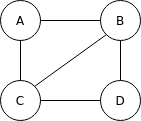
\includegraphics[width=5cm]{fig1}}
 	\caption{یک گراف بدون جهت شامل دو دور ساده}
 	\label{fig:fig1}
 \end{figure}
\subsection{پیدا کردن دور های ساده گراف}
پیدا کردن تمامی دور های ساده گراف از آن جهت برای ما اهمیت دارد که در مدل نهایی هر دور ساده
باعث یافتن یکی از
\LR{KVL}
موجود در مدار میشود.

برای یافتن مجموعه دور های ساده موجود در گراف ابتدا نیاز به یافتن درخت پوشای کمینه
\LTRfootnote{minimum spanning tree}
گراف یاد شده داریم، برای اینکار الگوریتم های زیادی از جمله الگوریتم کراسکال
\LTRfootnote{kruskal}
و الگوریتم پریم
\LTRfootnote{prim}
که در قسمت های
\ref{kruskal}
و
\ref{prim}
آمده است
طراحی شده اند، البته در پروژه حاضر از کتابخانه
\LR{networkx}
پایتون برای پیاده سازی استفاده شده است.

میتوان اثبات کرد که اگر یکی از یال های حذف شده را به درخت پوشای کمینه بیفزایم 
یک و تنها یک دور ساده ایجاد میشود که ما با الگوریتم
\LR{DFS}
که در قسمت
\ref{dfs}
آمده است
\LTRfootnote{depth first search}
آن دور را می یابیم
، سپس با افزودن تمامی یال ها به صورت تک به تک تمامی دور های ساده یافت میشود.

به عنوان نمونه اگه گراف شکل
\ref{fig:fig1}
ورودی ما باشد درخت پوشای کمینه ما شکل
\ref{fig:fig2}
خواهد بود که دارای دو یال قطع شده
\lr{AB}
و
\lr{BD}
است.که با نقطه چین نمایش داده شده اند.
با اضافه کردن یال های قطع شده به صورت تک به تک دو گراف شکل
\ref{fig:fig3}
پدید می آیند که هر کدام دارای دارای یک دور ساده هستند سپس همانطور که یاد شد
با الگوریتم
\lr{DFS}
دور های مورد نظر را می یابیم.
الگوریتم توضیح داده شده به صورت شبه کد در قسمت
\ref{simpcyc}
آمده است.
\cite{Dorfler18}
\begin{figure}[ht]
	\centerline{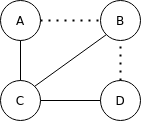
\includegraphics[width=5cm]{fig2}}
	\caption{درخت پوشای کمینه شکل
	\ref{fig:fig1} }
	\label{fig:fig2}
\end{figure}

\begin{figure}[ht]
	\centerline{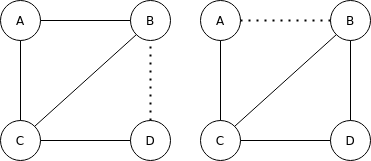
\includegraphics[width=9cm]{fig3}}
	\caption{دو گراف تک ساده دور شکل
		\ref{fig:fig1} }
	\label{fig:fig3}
\end{figure}
\begin{algorithm}[ht]
	\onehalfspacing
	\caption{الگوریتم پیدا کردن مجموعه دور های ساده گراف} 
	\label{simpcyc}
	\begin{algorithmic}[1]
		\REQUIRE
		\lr{graph}
		\ENSURE
		\lr{simple cycle entity}
		\STATE 
		\lr{create simple-cycles entity s = \{\}}
		\STATE 
		\lr{mst = kruskal(graph)}
		\STATE 
		\lr{store in stack s = graph - mst}
		\STATE
		\lr{store s.pop() in edge e}
		\STATE
		\lr{create new graph g = mst + e}
		\STATE
		\lr{define cycle c = dfs(g)}
		\STATE
		\lr{add cycle c to entity s }
		\STATE
		\lr{if stack s terminate the program otherwise return to instruction number4 }
	\end{algorithmic}
\end{algorithm}

\begin{algorithm}[ht]
	\onehalfspacing
	\caption{الگوریتم کراسکال} 
	\label{kruskal}
	\begin{algorithmic}[1]
		\REQUIRE
		\lr{graph}
		\ENSURE
		\lr{minimum spaning tree}
		\STATE
	    \lr{A = \{\}}
	    \STATE
	    \lr{For each vertex v in graph:}
	    \STATE
	    \lr{MAKE-SET(v)}
	    \STATE
		\lr{For each edge (u, v) in graph ordered by increasing order by weight(u, v):}
		\STATE
	    \lr{if FIND-SET(u) != FIND-SET(v):}
	    \STATE
	    \lr{A = A union (u, v)}
	    \STATE
	    \lr{UNION(u, v)}
	    \STATE
	    \lr{return A} 
	\end{algorithmic}
\end{algorithm}

\begin{algorithm}[ht]
	\onehalfspacing
	\caption{الگوریتم پریم} 
	\label{prim}
	\begin{algorithmic}[1]
		\REQUIRE
		\lr{graph}
		\ENSURE
		\lr{minimum spaning tree}
		\STATE
		\lr{A = \{\}}
		\STATE
		\lr{U = \{ 1 \}}
		\STATE
		\lr{while (U != V)}
		\STATE
		\lr{let (u, v) be the lowest cost edge such that u in U and v in V - U:}
		\STATE
		\lr{T = T union (u, v)}
		\STATE
		\lr{U = U union v}
				
	\end{algorithmic}
\end{algorithm}

\begin{algorithm}[ht]
	\onehalfspacing
	\caption{الگوریتم 
	\lr{dfs}
} 
	\label{dfs}
	\begin{algorithmic}[1]
		\REQUIRE
		\lr{graph}
		\ENSURE
		\lr{Stack S = \{\}}
		\STATE
		\lr{for each vertex u, set visited[u] = false}
		\STATE
		\lr{push v to S}
		\STATE
		\lr{while (S is not empty) do}
		\STATE
		\lr{u = S.pop()}
		\STATE
		\lr{while (S is not empty) do}
		\STATE
		\lr{if (not visited[u]) then}
		\STATE
		\lr{visited[u] := true}
		\STATE
		\lr{for each unvisited neighbour w of u}
		\STATE
		\lr{S.push(w)}
		
	\end{algorithmic}
\end{algorithm}

\section{جمع بندی}
در این فصل به مفاهیم نظریه گراف پرداخته شد که در فصل بعدی نقش اصلی را در مدل کردن مدار های الکتریکی به شکل انتزاعی بازی میکنند؛همانطور که پیشتر اشاره شد برای به دست آوردن پاسخ مدار ما نیازمند پیدا کردن تمامی قوانین
\lr{kvl}
هستیم، با در نظر گرفتن مدار به صورت گراف این مسئله به شکل یافتن تمامی دور های ساده گراف
در می آید که در الگوریتم
\eqref{simpcyc}
به آن پرداخته شده است.		% فصل سوم: روش تحقیق
% !TeX root=../main.tex
\chapter{جبر خطی}
%\thispagestyle{empty} 
\label{chap:results}
\section{پیشگفتار} 
ارائهٔ داده‌ها، نتایج، تحلیل و تفسیر اولیهٔ آنها در این فصل ارائه می‌شود. در ارائهٔ نتایج با توجه به راهنمای کلی نگارش فصل‌ها، تا حد امکان، ترکیبی از نمودار و جدول استفاده شود. با توجه به حجم و ماهیت تحقیق و با صلاحدید استاد راهنما، این فصل می‌تواند تحت عنوانی دیگر بیاید. در صورتی که حجم داده‌ها زیاد باشد، بهتر است به صورت نمودار یا در قالب ضمیمه ارائه نشده و فقط نمونه‌ها در متن آورده شود. در این فصل باید به سوالات تحقیق، عطف به یافته‌های محقق، پاسخ داده شود. اگر تحقیق دارای آزمون فرض باشد، پذیرش یا عدم پذیرش فرضیه‌ها در این فصل گزارش می‌شود. این فصل حدود ۴۰ صفحه است.

\section{محتوا}
در این بخش به سوالات تحقیق، بر اساس داده‌ها و یافته‌های محقق، پاسخ داده می‌شود. داده‌ها با فرمت مناسبی ارائه می‌شوند؛ مدل (ها) اجرا شده و نتیجه آن مشخص می‌شود.

\section{اعتبارسنجی}
از طریق مقایسهٔ نتایج با نتایج کارهای دیگران، استفاده از روش‌های تحلیل پایائی
\lr{(reliability)}
و اعتبار
\lr{(validity)}،
نظرگیری از خبرگان
\lr{(expert judgment or feedback)}
و یا
\lr{triangulation}
انجام می‌شود.
		% فصل چهارم: نتایج
% !TeX root=../main.tex
\chapter{اجرای برنامه}
\section{پیشگفتار} 
در این فصل تلاش میشود که شیوه اجرا برنامه و خروجی گرفتن از آن توضیح داده شود؛
لازم به یادآوریست همانطور که در پیشنهاده آمده است تمرکز این پروژه طراحی یک اپلیکیشن نیست و هدف تنها ارائه یک مدل ریاضی برای مدار های الکتریکی می باشد، همچنین به همین دلیل محیط
\lr{google colab}
برای برای تست کردن مدل انتخاب شده است.
\section{مخزن پروژه}
تمام برنامه ها و اسناد موجود برای این پروژه از طریق آدرس 
\href{https://github.com/Mehrdadghassabi/Gracc}{پیوند}
 شده قابل دسترسی است، همچنین در فایل
\lr{README.md}
توضیحات کوتاهی در مورد شیوه اجرا داده شده است، که البته در این فصل به توضیحات بیشتری پرداخته خواهد شد.
		% فصل پنجم: بحث و نتیجه‌گیری

% مراجع
% اگر از استیل‌های natbib استفاده می‌کنید باید دو خط را در فایل commands.tex تغییر دهید.
\pagestyle{empty}
{
\small
\onehalfspacing
\bibliographystyle{plain-fa} % or plainnat-fa for author-date
\bibliography{./tex/MyReferences}
}

\pagestyle{fancy}

% \appendix
% فصلهای پس از این قسمت به عنوان ضمیمه خواهند آمد.

% دستورات لازم برای تبدیل «فصل آ» به «پیوست آ» در فهرست مطالب
\addtocontents{toc}{
    \protect\renewcommand\protect\cftchappresnum{\appendixname~}%
    \protect\setlength{\cftchapnumwidth}{\mylenapp}}
    
% دستورات لازم برای شماره‌گذاری صفحات پیوست‌ها بشکل آ-۱ (فعلا با glossaries سازگار نیست)
% \let\Chapter\chapter
%\pretocmd{\chapter}{
%  \clearpage
%  \pagenumbering{arabic}
%  \renewcommand*{\thepage}{\rl{\thechapter-\arabic{page}}}}{}{}
%%%%%%%%%%%%%%%%%%%%%%%%%%%%%%%%%%%%%
        

% !TeX root=../main.tex

\chapter{آشنایی سریع با برخی دستورات لاتک}
\label{app:latexIntro}
%\thispagestyle{empty}
در این فصل ویژگی‌های مهم و پرکاربرد زی‌پرشین و لاتک معرفی می‌شود. برای راهنمایی بیشتر و به‌کاربردن ویژگی‌های پیشرفته‌تر به راهنمای زی‌پرشین و راهنمای لاتک مراجعه کنید. برای آگاهی از دستورات لاتک که این خروجی را تولید کرده‌اند فایل \lr{appendix1.tex} را ملاحظه فرمایید.
\footnote{بیشتر مطالب این بخش از مثال 
\lr{xepersian\_example.tex}
گرفته شده‌اند که توسط آقای امیرمسعود پورموسی آماده شده است.}

\section{بندها و زیرنویس‌ها}
هر جایی از نوشتهٔ خود، اگر می‌خواهید به سر سطر بروید و یک بند (پاراگراف) تازه را آغاز کنید، باید یک خط را خالی بگذارید%
\footnote{یعنی دوبار باید کلید \lr{Enter} را بزنید.}
 مانند این:

حالا که یک بند تازه آغاز شده است، یک زیرنویس انگلیسی%
\LTRfootnote{English Footnote!}
 هم می‌نویسیم!
\section{فرمول‌های ریاضی}
\label{formula}

اینجا هم یک فرمول می‌آوریم که شماره دارد:
\begin{equation}\label{eq:yek}
A=\frac{c}{d}+\frac{q^2}{\sin(\omega t)+\Omega_{12}}
\end{equation}
در لاتک می‌توان به کمک فرمان 
\lr{\textbackslash label\{\}}
به هر فرمول یک نام نسبت داد. در فرمول بالا نام \lr{eq:yek} را برایش گذاشته‌ایم (پروندهٔ \lr{tex} همراه با این مثال را ببینید). این نام ما را قادر می‌کند که بعداً بتوانیم با فرمان
\lr{\textbackslash ref\{eq:yek\}}
به آن فرمول با شماره ارجاع دهیم. یعنی بنویسیم فرمول \ref{eq:yek}. 
لاتک خودش شمارهٔ این فرمول‌ها را مدیریت می‌کند.\footnote{یعنی اگر بعداً فرمولی قبل از این فرمول بنویسیم، خودبه‌خود شمارهٔ این فرمول و شمارهٔ ارجاع‌ها به این فرمول یکی زیاد می‌شود. دیگر نگران شماره‌گذاری فرمول‌های خود نباشید!} این هم یک فرمول که شماره ندارد:
$$A=|\vec{a}\times \vec{b}| + \sum_{n=0}^\infty C_{ij}$$

این هم عبارتی ریاضی مانند 
$\sqrt{a^2+b^2}$
 که بین متن می‌آید.
\subsection{یک زیربخش}
\label{zirbakhsh}

این زیربخش \ref{zirbakhsh} است؛ یعنی یک بخش درون بخش \ref{formula} است.
\subsubsection{یک زیرزیربخش}
این هم یک زیرزیربخش است. در لاتک می‌توانید بخش‌های تودرتو در نوشته‌تان تعریف کنید تا ساختار منطقی نوشته را به خوبی نشان دهید. می‌توانید به این بخش‌ها هم با شماره ارجاع دهید، مثلاً بخش فرمول‌های ریاضی شماره‌اش \ref{formula} است.
\section{نوشته‌های فارسی و انگلیسی مخلوط}
نوشتن یک کلمهٔ انگلیسی بین متن فارسی بدیهی است، مانند Example در این جمله.\footnote{هرچند بهتر است باز هم آن کلمه را مانند \lr{Example} در این جمله بنویسید.}
نوشتن یک عبارت چندکلمه‌ای مانند
 \lr{More than one word} کمی پیچیده‌تر است.

اگر ناگهان تصمیم بگیرید که یک بند کاملاً انگلیسی را بنویسید، باید:
\begin{latin}
This is an English paragraph from left to right. You can write as much as you want in it.
\end{latin}
\section{افزودن تصویر به نوشته}
پروندهٔ تصویر دلخواه خود را در کنار پروندهٔ \lr{tex} قرار دهید. سپس به روش زیر تصویر را در نوشتهٔ خود بیاورید:
\begin{latin}
\begin{verbatim}
\includegraphics{YourImageFileName}
\end{verbatim}
\end{latin}
به تصویرها هم مانند فرمول‌ها و بخش‌ها می‌توان با شماره ارجاع داد. مثلاً تصویر \ref{fig:shir} یک شیر علاقه‌مند به لاتک را در حال دویدن نشان می‌دهد. برای جزئیات بیشتر دربارهٔ روش گذاشتن تصویرها در نوشته باید راهنماهای لاتک را بخوانید.
\begin{figure}[ht]
\centerline{
\includegraphics[width=5cm]{logo}}
\caption{در این تصویر یک شیر علاقه‌مند به لاتک را در حال دویدن می‌بینید.}
\label{fig:shir}
\end{figure}

به تصویرها هم مانند فرمول‌ها و بخش‌ها می‌توان با شماره ارجاع داد. مثلاً تصویر بالا شماره‌اش \ref{fig:shir} است. برای جزئیات بیشتر دربارهٔ روش گذاشتن تصویرها در نوشته باید راهنماهای لاتک را بخوانید.

\section{محیط‌های شمارش و نکات}
برای فهرست‌کردن چندمورد، اگر ترتیب برایمان مهم نباشد:
\begin{itemize}
\item مورد یکم
\item مورد دوم
\item مورد سوم
\end{itemize}
و اگر ترتیب برایمان مهم باشد:
\begin{enumerate}
\item مورد یکم
\item مورد دوم
\item مورد سوم
\end{enumerate}
می‌توان موردهای تودرتو داشت:
\begin{enumerate}
\item مورد ۱
\item مورد ۲
\begin{enumerate}
\item مورد ۱ از ۲
\item مورد ۲ از ۲
\item مورد ۳ از ۲
\end{enumerate}
\item مورد ۳
\end{enumerate}
شماره‌گذاری این موردها را هم لاتک انجام می‌دهد.

\section{تعریف و قضیه}
برای ذکر تعریف، قضیه و مثال مثالهای ذیل را ببینید.
\begin{definition}
مجموعه همه ارزیابی‌های  (پیوسته)  روی $(X,\tau)$، دامنه توانی احتمالی
\index{دامنه توانی احتمالی}
$ X $
نامیده می‌شود.
\end{definition}
\begin{theorem}[باناخ-آلااغلو]
\index{قضیه باناخ-آلااغلو}
اگر $ V $ یک همسایگی $ 0 $ در فضای برداری 
\index{فضای!برداری}
 توپولوژیکی $ X $ باشد و 
\begin{equation}\label{eq1}
K=\left\lbrace \Lambda \in X^{*}:|\Lambda x|\leqslant 1 ; \ \forall x\in V\right\rbrace,
\end{equation}
آنگاه $ K $،  ضعیف*-فشرده است که در آن، $ X^{*} $ دوگان
\index{فضای!دوگان}
 فضای برداری توپولوژیکی $ X $ است به ‌طوری که عناصر آن،  تابعی‌های 
خطی پیوسته
\index{تابعی خطی پیوسته}
 روی $X$ هستند.
\end{theorem}
تساوی \eqref{eq1} یکی از مهم‌ترین تساوی‌ها در آنالیز تابعی است که در ادامه، به وفور از آن استفاده می‌شود.
\begin{example}
برای هر فضای مرتب، گردایه 
$$U:=\left\lbrace U\in O: U=\uparrow U\right\rbrace $$
از مجموعه‌های بالایی باز، یک توپولوژی تعریف می‌کند که از توپولوژی اصلی، درشت‌تر  است.
\end{example}
حال تساوی 
\begin{equation}\label{eq2}
\sum_{n=1}^{+\infty} 3^{n}x+7x=\int_{1}^{n}8nx+\exp{(2nx)}
\end{equation}
را در نظر بگیرید. با مقایسه تساوی \eqref{eq2} با تساوی \eqref{eq1} می‌توان نتیجه گرفت که ...


\section{چگونگی نوشتن و ارجاع به مراجع}
\label{Sec:Ref}


در لاتک به راحتی می‌توان مراجع خود را نوشت و به آنها ارجاع داد. به عنوان مثال برای معرفی کتاب گنزالس \cite{Gonzalez02book} به عنوان یک مرجع می‌توان آنرا به صورت زیر معرفی نمود:

\singlespacing
\begin{LTR}
\begin{verbatim}
\bibitem{Gonzalez02book}
Gonzalez, R.C., and Woods, R.E. {\em Digital Image Processing}, 3rd ed..
Prentice-Hall, Inc., Upper Saddle River, NJ, USA, 2006.
\end{verbatim}
\end{LTR}
\doublespacing

در دستورات فوق \lr{Gonzalez02book}  برچسبی است که به این مرجع داده شده است و با استفاده از دستور 
\verb!\cite{Gonzalez02book}!
می‌توان به آن ارجاع داد؛ بدون این که شماره‌اش را در فهرست مراجع‌مان بدانیم.

اگر این اولین مرجع ما باشد در قسمت مراجع به صورت زیر خواهد آمد:\\
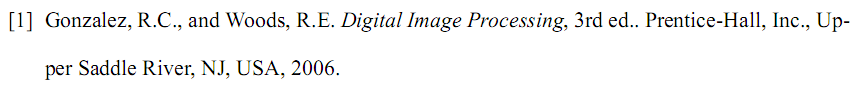
\includegraphics[width=\textwidth]{gonzalez.png}

این شیوهٔ تعریف مراجع بسیار ابتدایی است و اگر فرمت مراجع، ترتیب یا تعداد آنها را خواسته باشید تغییر دهید، به عنوان مثال ابتدا حرف اول نام نویسنده بیاید و سپس نام خانوادگی، باید همه کارها را به صورت دستی انجام دهید!
چون در یک \پ یا مقاله باید کنترل کاملی بر مراجع خود داشته باشید و به راحتی بتوانید قالب مراجع را عوض کنید، بنابراین می‌بایست از \lr{Bib\TeX} استفاده کنید که درپیوست  \ref{app:refMan} به  آن پرداخته خواهد شد.
		% پیوست اول: آشنایی مقدماتی با لاتک
% !TeX root=../main.tex

\chapter{‌جدول، نمودار و الگوریتم در لاتک}
\label{app:latex:more}
%\thispagestyle{empty}

در این بخش نمونه مثالهایی از جدول، شکل، نمودار، الگوریتم و معادلات ریاضی را در لاتک خواهیم دید.
دقت کنید که در پایان‌نامه‌ها و مقالات، باید قاعدهٔ «ارجاع به جلو%
\LTRfootnote{Forward Referencing}»
رعایت شود؛ یعنی ابتدا در متن به شمارهٔ شکل، جدول یا معادله اشاره شود و بعد از آن (زیر آن) خود شکل، جدول یا معادله رسم شود. (توضیحات بیشتر در قسمت
\ref{sec:floatObjs}).

\section{جدول}
دستور اصلی برای رسم جدول در لاتک 
\verb|tabular|
می‌باشد که جدول
\eqref{tab:motionModels}
با استفاده از آن کشیده شده است؛ در
\verb|tabular|
عرض جدول برابر با مجموع عرض ستون‌ها و حداکثر مساوی عرض متن است.
\begin{table}[ht]
\caption{مدلهای تبدیل.}
\label{tab:motionModels}
\centering
\onehalfspacing
\begin{tabular}{|r|c|l|r|}
	\hline نام مدل & درجه آزادی & تبدیل مختصات & توضیح \\ 
	\hline انتقالی & ۲ & $\begin{aligned} x'=x+t_x \\ y'=y+t_y \end{aligned}$  &  انتقال دوبعدی\\ 
	\hline اقلیدسی & ۳ & $\begin{aligned} x'=x\cos\theta - y\sin\theta+t_x \\ y'=x\sin\theta+y\cos\theta+t_y \end{aligned}$  &  انتقالی+دوران \\ 
	\hline 
\end{tabular} 
\end{table}

برای اینکه عرض جدول قابل کنترل باشد، باید از دستورات
\verb|tabularx|،
\verb|tabulary| یا
\verb|tabu|
استفاده کرد که راهنمای آنها در اینترنت وجود دارد.
مثلاً جدول
\ref{tab:motionModelsCont}
با
\verb|tabularx|
رسم شده که عرض جدول در آن ثابت بوده و ستون‌های از نوع
\verb|X|
عرض خالی جدول را پر می‌کنند.
\begin{table}[ht]
	\caption{مدلهای تبدیل دیگر.}
	\label{tab:motionModelsCont}
	\centering
	\onehalfspacing
	\begin{tabularx}{\textwidth}{|r|c|l|X|}
		\hline نام مدل & درجه آزادی & تبدیل مختصات & توضیح \\ 
		\hline مشابهت & ۴ & $\begin{aligned} x'=sx\cos\theta - sy\sin\theta+t_x \\ y'=sx\sin\theta+sy\cos\theta+t_y  \end{aligned}$  & اقلیدسی+تغییرمقیاس \\ 		
		\hline آفین & ۶ & $\begin{aligned} x'=a_{11}x+a_{12}y+t_x \\ y'=a_{21}x+a_{22}y+t_y \end{aligned}$  & مشابهت+اریب‌شدگی \\
		\hline
	\end{tabularx}
\end{table}

\section{معادلات ریاضی و ماتریس‌ها}
تقریباً هر آنچه دانشجویان برای نوشتن فرمول‌های ریاضی لازم دارند، در کتاب 
\lr{mathmode}
آمده است. کافیست در خط فرمان، دستور زیر را وارد کنید:
\begin{latin}
	\texttt{texdoc mathmode}
\end{latin}
متن زیر شامل انواعی از اشیاء ریاضی است که با ملاحظه کدش می‌توانید با دستورات آن آشنا شوید.\\
شناخته‌شده‌ترین روش تخمین ماتریس هوموگرافی الگوریتم تبدیل خطی مستقیم (\lr{DLT\LTRfootnote{Direct Linear Transform}}) است.  فرض کنید چهار زوج نقطهٔ متناظر در دو تصویر در دست هستند،  $\mathbf{x}_i\leftrightarrow\mathbf{x}'_i$   و تبدیل با رابطهٔ
  $\mathbf{x}'_i = H\mathbf{x}_i$
  نشان داده می‌شود که در آن:
\[\mathbf{x}'_i=(x'_i,y'_i,w'_i)^\top  \]
و
\[ H=\left[
\begin{array}{ccc}
h_1 & h_2 & h_3 \\ 
h_4 & h_5 & h_6 \\ 
h_7 & h_8 & h_9
\end{array} 
\right]\]
رابطه زیر را برای الگوریتم  \eqref{alg:DLT} لازم داریم.
\begin{equation}
\label{eq:DLT_Ah}
\left[
\begin{array}{ccc}
	0^\top & -w'_i\mathbf{x}_i^\top & y'_i\mathbf{x}_i^\top \\ 
	w'_i\mathbf{x}_i & 0^\top & -x'_i\mathbf{x}_i^\top \\ 
	- y'_i\mathbf{x}_i^\top & x'_i\mathbf{x}_i^\top & 0^\top
\end{array} 
\right]
\left(
\begin{array}{c}
	\mathbf{h}^1 \\ 
	\mathbf{h}^2 \\ 
	\mathbf{h}^3
\end{array} 
\right)=0
\end{equation}

\section{الگوریتم}

\subsection{الگوریتم ساده با دستورهای فارسی}
با مفروضات فوق، الگوریتم \lr{DLT} به صورت نشان داده شده در الگوریتم \eqref{alg:DLT}  خواهد بود.
\begin{algorithm}[ht]
\onehalfspacing
\caption{الگوریتم \lr{DLT} برای تخمین ماتریس هوموگرافی.} \label{alg:DLT}
\begin{algorithmic}[1]
\REQUIRE $n\geq4$ زوج نقطهٔ متناظر در دو تصویر 
${\mathbf{x}_i\leftrightarrow\mathbf{x}'_i}$،\\
\ENSURE ماتریس هوموگرافی $H$ به نحوی‌که: 
$\mathbf{x}'_i = H \mathbf{x}_i$.
  \STATE برای هر زوج نقطهٔ متناظر
$\mathbf{x}_i\leftrightarrow\mathbf{x}'_i$ 
ماتریس $\mathbf{A}_i$ را با استفاده از رابطهٔ \ref{eq:DLT_Ah} محاسبه کنید.
  \STATE ماتریس‌های ۹ ستونی  $\mathbf{A}_i$ را در قالب یک ماتریس $\mathbf{A}$ ۹ ستونی ترکیب کنید. 
  \STATE تجزیهٔ مقادیر منفرد \lr{(SVD)}  ماتریس $\mathbf{A}$ را بدست آورید. بردار واحد متناظر با کمترین مقدار منفرد جواب $\mathbf{h}$ خواهد بود.
  \STATE  ماتریس هوموگرافی $H$ با تغییر شکل $\mathbf{h}$ حاصل خواهد شد.
\end{algorithmic}
\end{algorithm}

\subsection{الگوریتم پیچیده و تودرتو با دستورهای فارسی}
الگوریتم \ref{alg:simulation-random}، یک الگوریتم ترکیبی و تودرتو است که با کمک دستورهای بستهٔ \lr{algorithmic} نوشته شده است.

\begin{algorithm}[p]
    \onehalfspacing
    \caption{الگوریتم اجرای برنامهٔ شبیه‌سازی}
    \label{alg:simulation-random}
    \begin{algorithmic}[1]
        \REQUIRE زمان $t_{max}$ به عنوان زمان لازم برای انجام شبیه سازی،\\
        \REQUIRE  گراف شبکه برای شبیه سازی،
        \ENSURE جدول تغییرات گراف از لحظهٔ ۰ تا t.
        \FOR {تمام لحظات در بازهٔ ۰ تا $t_{max}$}
            \FOR {تمام پیوند‌ها}
                \STATE محاسبهٔ ضریب و نرخ انتقال پیوند
                \STATE محاسبهٔ کیفیت و نرخ یادگیری
            \ENDFOR
            \FOR {تمام گره‌ها}
                \STATE محاسبهٔ نرخ انتقال گره
                \STATE محاسبهٔ وضعیت جدید
            \ENDFOR
            \IF {تغییرات از مقدار $\delta$ کمتر است}
                \STATE شکستن حلقه
                \COMMENT{این شرط برای پایان قبل از رسیدن به محدودیت زمانی است، اگر تغییرات کمتر از $\delta$ باشد}
            \ELSIF {زمان اجرای برنامه بیش از حد طول کشیده \AND $t>100$}
                \STATE شکستن حلقه
            \ENDIF
        \ENDFOR
        \PRINT {زمان اجرای برنامه}
        \RETURN {ماتریس تغییرات زمانی}
    \end{algorithmic}
\end{algorithm}

\subsection{الگوریتم با دستورهای لاتین}
الگوریتم \ref{alg:RANSAC} یک الگوریتم با دستورهای لاتین است.

\begin{algorithm}[ht]
\onehalfspacing
\caption{الگوریتم \lr{RANSAC} برای تخمین ماتریس هوموگرافی.} \label{alg:RANSAC}
\begin{latin}
\begin{algorithmic}[1]
\REQUIRE $n\geq4$ putative correspondences, number of estimations, $N$, distance threshold $T_{dist}$.\\
\ENSURE Set of inliers and Homography matrix $H$.
\FOR{$k = 1$ to $N$}
  \STATE Randomly choose 4 correspondence,
  \STATE Check whether these points are colinear, if so, redo the above step
  \STATE Compute the homography $H_{curr}$ by DLT algorithm from the 4 points pairs,
  \STATE $\ldots$ % الگوریتم کامل نیست
  \ENDFOR
  \STATE Refinement: re-estimate H from all the inliers using the DLT algorithm.
\end{algorithmic}
\end{latin}
\end{algorithm}

\section{کد}
درج کد به زبان‌های مختلف به سادگی امکان‌پذیر است. برنامه
\ref{code:matlabEx}
یک قطعه کد
\lr{MATLAB}
را نشان می‌دهد.
\begin{figure}[ht]
	\begin{LTR}
        \singlespacing
		\lstinputlisting[language=MATLAB, caption={نمونه کد \lr{MATLAB}}, label={code:matlabEx}]{MatlabExample.m}
        % \doublespacing
	\end{LTR}
\end{figure}

\section{تصویر}
نمونهٔ یک تصویر را در فصل قبل دیدیم. دو تصویر شیر کنار هم را نیز در شکل
\ref{fig:twoLion}
مشاهده می‌کنید.
\begin{figure}[ht]
\centering 
\subfloat[شیر ۱]{ \label{fig:twolion:one}

\includegraphics[width=0.3\textwidth]{lion}}
%\hspace{2mm}
\subfloat[شیر ۲]{ \label{fig:twolion:two}

\includegraphics[width=0.3\textwidth]{lion}}%
\caption{دو شیر}
\label{fig:twoLion} %% label for entire figure
\end{figure}

\section{نمودار}
لاتک بسته‌هایی با قابلیت‌های زیاد برای رسم انواع مختلف نمودارها دارد. مانند بسته‌های \lr{Tikz} و  \lr{PSTricks}. توضیح اینها فراتر از این پیوست کوچک است.%
\footnote{
مثال‌هایی از بکارگیری بسته
\lr{Tikz}
را می‌توانید در
\url{http://www.texample.net/tikz/examples/}
ببینید. توصیه می‌شود دانشجویانی که قصد درج اشکالی مانند گراف را در سند خود دارند، مثالهایی از سایت مذکور را ملاحظه فرمایند.
}
یک نمودار رسم شده با بستهٔ 
\lr{TikZ}
 در شکل 
\ref{fig:parabola}
نشان داده شده است.
\begin{figure}[t]
\centering
\begin{tikzpicture}[scale=2.5]
  \shade[top color=blue,bottom color=gray!50] 
      (0,0) parabola (1.5,2.25) |- (0,0);
  \draw (1.05cm,2pt) node[above] 
      {$\displaystyle\int_0^{3/2} \!\!x^2\mathrm{d}x$};

  \draw[style=help lines] (0,0) grid (3.9,3.9)
       [step=0.25cm]      (1,2) grid +(1,1);

  \draw[->] (-0.2,0) -- (4,0) node[right] {$x$};
  \draw[->] (0,-0.2) -- (0,4) node[above] {$f(x)$};

  \foreach \x/\xtext in {1/1, 1.5/1\frac{1}{2}, 2/2, 3/3}
    \draw[shift={(\x,0)}] (0pt,2pt) -- (0pt,-2pt) node[below] {$\xtext$};

  \foreach \y/\ytext in {1/1, 2/2, 2.25/2\frac{1}{4}, 3/3}
    \draw[shift={(0,\y)}] (2pt,0pt) -- (-2pt,0pt) node[left] {$\ytext$};

  \draw (-.5,.25) parabola bend (0,0) (2,4) node[below right] {$x^2$};
\end{tikzpicture}
\caption{یک نمودار زیبا با ارقام فارسی و قابلیت بزرگ‌نمایی بسیار، بدون از دست دادن کیفیت.}
\label{fig:parabola}
\end{figure}

\section{نحوه قرارگیری اشیای شناور}
\label{sec:floatObjs}
شکل‌ها، جداول و الگوریتم‌ها در لاتک اشیای شناور محسوب می‌شوند؛ یعنی خود لاتک تصمیم می‌گیرد آنها را در کجای صفحه ترسیم کند تا زیباتر باشد. اما می‌توان به لاتک توصیه کرد که آن را در قسمت خاصی از صفحه رسم کند. برای اینکه قاعدهٔ «ارجاع به جلو» رعایت شود باید فقط از پرچم
\verb|[ht]|
استفاده کرد، که می‌گوید اگر جا شد شکل را دقیقاً در همین مکان و در غیراینصورت در بالای صفحه بعد رسم کن.
بنابراین دستورات درج تصویر، جدول و الگوریتم به صورت زیر باید باشند:

\begin{latin}
\begin{verbatim}
	\begin{figure/table/algorithm}[ht]
		...
	\end{figure/table/algorithm}
\end{verbatim}
\end{latin}
		% پیوست دوم: جدول، نمودار و الگوریتم در لاتک
% !TeX root=../main.tex
\begin{thebibliography}{9}
	\bibitem{Stella15}
	\lr{
	L Toscano, S Stella and E Milotti (2015) Using graph theory for automated electric circuit solving,italy European Journal of Physics}
	
	\bibitem{Isabel20}
	\lr{
		Julie Isabel Arago Delage (2020) ELECTRICAL CIRCUIT
		SIMULATION, universitat de barcelona Facultat de matematiques i informatica.}
	
	\bibitem{Dorfler18}
	\lr{
		F Dorfler,J W Simpson-Porco,F  Bullo (2018) Electrical Networks and Algebraic Graph Theory: Models, Properties, and Applications, IEEE}
	
	\bibitem{Mahoney15}
	\lr{
		M mahoney (2015) Modeling graphs with electrical networks, university of berkeley}
	
	\bibitem{Berdewad14}
	\lr{
		Berdewad O. K., Dr. Deo S. D (2014) Application of Graph Theory in Electrical Network, gondwana university}
	
	\bibitem{thulasiraman02}
	\lr{
		K thulasiraman (2002) circuit theory, university of oklahama}
	
	\bibitem{mirzaee14}
	\lr{
		F mirzaee, S bismel (2014) A new Euler matrix method for solving systems of linear Volterra integral equations with variable coefficients, Egyptian Mathematical}
	
	\bibitem{Alexander13}
	\lr{
		Charles K. Alexander and Matthew N.O. Sadiku (2013) Fundamentals of Electric
		Circuits, New York McGraw-Hill}
	
\end{thebibliography}   	% پیوست سوم: مراجع، واژه‌نامه و حاشیه‌نویسی

% برگرداندن شماره‌بندی صفحات فصول
% \let\chapter\Chapter
\pagenumbering{tartibi} % اول، دوم، ...
%\baselineskip=.75cm

% چاپ واژه‌نامه‌ها و نمایه 
\onehalfspacing
\cleardoublepage
\printglossary
\cleardoublepage
\printindex



\end{document}
